\documentclass[12pt,a4paper]{report}

\usepackage[margin=1in]{geometry}
\usepackage{graphicx}
\usepackage{array}
\usepackage{booktabs}
\usepackage{float}
\usepackage{setspace}
\usepackage{titlesec}
\usepackage{tocloft}
\usepackage{enumitem}
\usepackage{hyperref}
\usepackage{xcolor}
\usepackage{url}
\usepackage{eso-pic}
\usepackage{tikz}
\usepackage{fancyhdr}
\usepackage{lastpage}
\usepackage{etoolbox}

\hypersetup{
    colorlinks=true,
    linkcolor=black,
    urlcolor=blue,
    pdftitle={Internship Report},
    pdfauthor={Kamal S}
}

% -- Spacing ----------------------------------------------------------------
\setstretch{1.5}
\setlength{\parindent}{1.5em}
\setlength{\parskip}{0.4em}

% -- Chapter heading format -------------------------------------------------
\\titleformat{\\chapter}[display]
  {\\bfseries\\Large}
  {\\chaptername~\\thechapter}{10pt}{\\LARGE\\markboth{\\MakeUppercase{##1}}{\\MakeUppercase{##1}}}

% Ensure chapter marks are set for headers
\\renewcommand{\\chaptermark}[1]{\\markboth{##1}{##1}}

% -- Rename TOC / LOF headings to match template ----------------------------
\renewcommand{\contentsname}{TABLE OF CONTENTS}
\renewcommand{\listfigurename}{}

% -- TOC heading format (consistent with other front-matter headings) -------
\renewcommand{\cfttoctitlefont}{\hfill\LARGE\bfseries}
\renewcommand{\cftaftertoctitle}{\hfill}
\renewcommand{\cftloftitlefont}{\hfill\LARGE\bfseries}
\renewcommand{\cftafterloftitle}{\hfill}
\setlength{\cftbeforetoctitleskip}{0pt}
\setlength{\cftaftertoctitleskip}{1.5em}

% -- Toggle: border ON/OFF --------------------------------------------------
% We define a boolean that controls whether borders are drawn.
% Front-matter pages: border ON.  Chapter pages: border OFF.
\newif\ifshowborder
\showbordertrue  % start with borders ON

\AddToShipoutPictureBG{%
  \ifshowborder
  \begin{tikzpicture}[remember picture, overlay]
    \draw[line width=0.56pt]
      ([xshift=18pt, yshift=-18pt]current page.north west)
      rectangle
      ([xshift=-18pt, yshift=18pt]current page.south east);
    \draw[line width=0.28pt]
      ([xshift=20pt, yshift=-20pt]current page.north west)
      rectangle
      ([xshift=-20pt, yshift=20pt]current page.south east);
  \end{tikzpicture}%
  \fi
}

% -- Page styles ------------------------------------------------------------

% Style for front-matter: no header/footer, just centered page number
\fancypagestyle{frontmatter}{
  \fancyhf{}
  \renewcommand{\headrulewidth}{0pt}
  \renewcommand{\footrulewidth}{0pt}
  \fancyfoot[C]{\thepage}
}

% Style for main content: header + footer, no border
\fancypagestyle{mainchapter}{
  \fancyhf{}
  \renewcommand{\headrulewidth}{0.4pt}
  \renewcommand{\footrulewidth}{0.4pt}
  \fancyhead[L]{\small FullStack developer}
  \fancyhead[R]{\small\nouppercase{\leftmark}}
  \fancyfoot[L]{\small Dept. of ECE, Vemana IT}
  \fancyfoot[C]{\small 2025-2026}
  \fancyfoot[R]{\small Page \thepage\ of \pageref{LastPage}}
}

% Plain style for front-matter (used by \chapter*, \listoffigures, etc.)
% Initially just centered page number. Redefined before main content.
\fancypagestyle{plain}{
  \fancyhf{}
  \renewcommand{\headrulewidth}{0pt}
  \renewcommand{\footrulewidth}{0pt}
  \fancyfoot[C]{\thepage}
}

\begin{document}

% ==========================================================================
% TITLE PAGE  (single-spaced, zero parskip so it fits on one page)
% ==========================================================================
\begin{titlepage}
\thispagestyle{empty}
\begin{singlespacing}
\setlength{\parskip}{0pt}
\setlength{\parindent}{0pt}
\centering
\vspace*{-0.5cm}

{\Large \textbf{VISVESVARAYA TECHNOLOGICAL UNIVERSITY}\par}
\vspace{2pt}
{\large \textbf{Jnana Sangama, Belagavi -- 590018}\par}
\vspace{8pt}

\includegraphics[height=5cm]{images/vtu_logo.png}\par
\vspace{8pt}
{\itshape An Internship Report\par}
\vspace{2pt}
{\itshape On\par}
\vspace{4pt}
{\LARGE \textbf{\textquotedblleft FullStack developer\textquotedblright}\par}
\vspace{4pt}
{\textcolor{red}{Jan 27 to April 27}\par}
\vspace{8pt}
{\itshape Submitted in partial fulfillment of the requirements for the award of the degree of\par}
\vspace{4pt}
{\large \textbf{Bachelor of Engineering}\par}
\vspace{2pt}
{\large \textbf{in}\par}
\vspace{2pt}
{\large \textbf{\textcolor{blue}{Electronics and communications}}\par}
\vspace{8pt}
Submitted by\par
\vspace{4pt}
{\large \textbf{KAMAL S \hspace{2cm} 1VI22EC066}\par}
\vspace{10pt}

\includegraphics[height=4cm]{images/vit_logo.png}\par
\vspace{10pt}
{\large \textbf{DEPARTMENT OF ELECTRONICS AND COMMUNICATIONS}\par}
{\Large \textbf{VEMANA INSTITUTE OF TECHNOLOGY}\par}
{\large BENGALURU -- 560034\par}
\vspace{6pt}
{\Large \textbf{2025-2026}\par}

\end{singlespacing}
\end{titlepage}

% ==========================================================================
% FRONT MATTER — borders ON, roman numbering, no headers/footers
% ==========================================================================
\pagenumbering{roman}
\pagestyle{frontmatter}

% ==========================================================================
% CERTIFICATE PAGE
% ==========================================================================
\thispagestyle{empty}
\begin{singlespacing}
\setlength{\parskip}{0pt}
\setlength{\parindent}{0pt}
\begin{center}
{\large \textbf{Karnataka ReddyJana Sangha}\par}
\vspace{2pt}
{\Large \textbf{VEMANA INSTITUTE OF TECHNOLOGY}\par}
\vspace{2pt}
(Affiliated to Visvesvaraya Technological University, Belagavi)\par
Koramangala, Bengaluru--560034\par
\vspace{8pt}

\includegraphics[height=3.5cm]{images/dept_seal.png}\par
\vspace{10pt}
{\large \textbf{DEPARTMENT OF}\par}
{\large \textbf{ELECTRONICS AND COMMUNICATIONS}\par}
\vspace{10pt}
{\LARGE \textbf{CERTIFICATE}\par}
\end{center}
\end{singlespacing}

\vspace{6pt}
\setlength{\parindent}{1.5em}
This is to certify that the internship entitled \textbf{\textquotedblleft FullStack developer\textquotedblright} is a bonafide work carried out by \textbf{KAMAL S (1VI22EC066)} in partial fulfilment of the requirements for the award of Bachelor of Engineering degree in \textbf{Electronics and communications}, Visvesvaraya Technological University, Belagavi, during the academic year 2025-2026.

It is certified that all corrections and suggestions indicated for internal assessment have been duly incorporated in the report. The internship report has been approved as it satisfies the academic requirements prescribed for the said degree.

% -- Watermark: VIT logo behind signatures ---------------------------------
\AddToShipoutPictureFG*{%
  \begin{tikzpicture}[remember picture, overlay]
    \node[opacity=0.10] at ([yshift=-4cm]current page.center) {%
      
\includegraphics[height=8cm]{images/vit_logo.png}%
    };
  \end{tikzpicture}%
}

\vspace{0.6cm}
\begin{center}
\begin{tabular}{p{0.22\textwidth} p{0.22\textwidth} p{0.22\textwidth} p{0.22\textwidth}}
\textbf{Internal Supervisor} & \textbf{External Supervisor} & \textbf{HOD} & \textbf{Principal} \\
(Prof. Suma B V) & (Maneesh Kumar Varma) & (Dr. Suneeta) & (Dr. Vijayasimha Reddy B G) \\
\end{tabular}
\end{center}

\vspace{0.5cm}
\textbf{Name of the Examiners} \hfill \textbf{Signature with Date}\par
\vspace{0.2cm}
1.\enspace\rule{5cm}{0.4pt} \hfill \rule{3.5cm}{0.4pt}\par
\vspace{0.4cm}
2.\enspace\rule{5cm}{0.4pt} \hfill \rule{3.5cm}{0.4pt}\par


\newpage
\begin{center}
\vspace*{\fill}
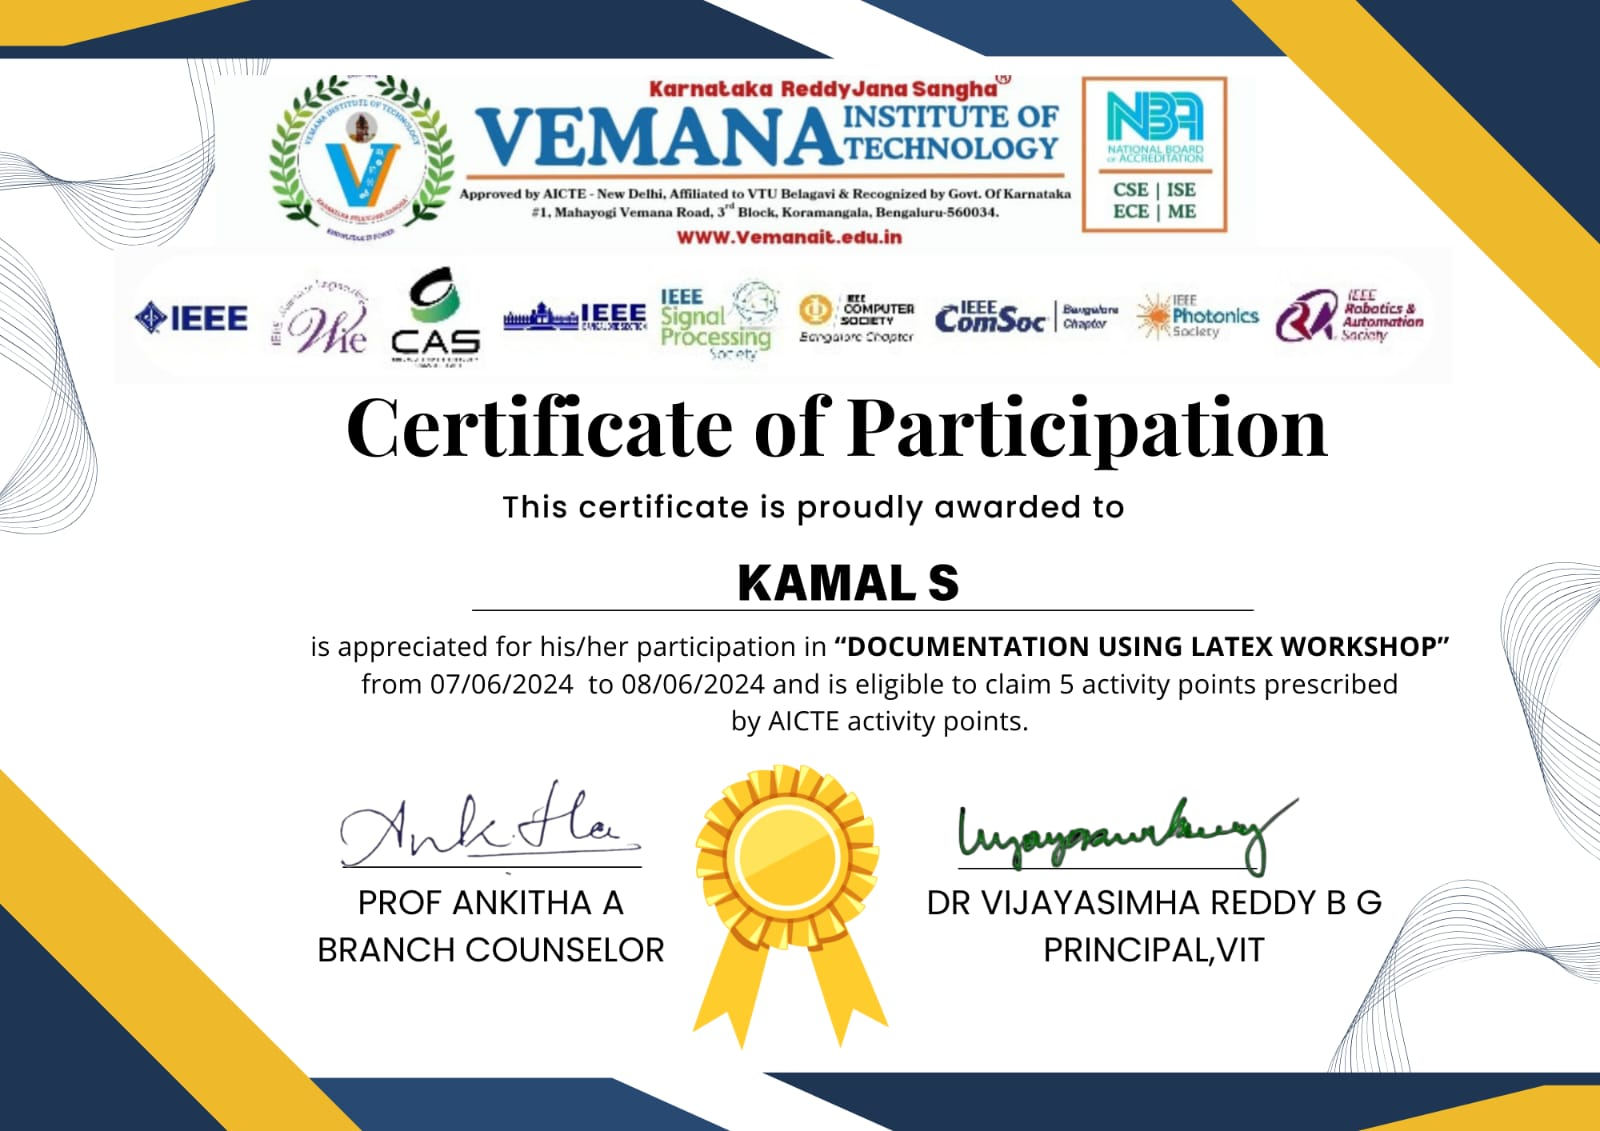
\includegraphics[angle=90,origin=c,width=0.92\textheight,height=0.92\textwidth,keepaspectratio]{images/cert_image_7d09766c.jpeg}
\vspace*{\fill}
\end{center}


% ==========================================================================
% ACKNOWLEDGEMENT
% ==========================================================================
\newpage
\setcounter{page}{2}  % Ack = page ii (certificate was empty)
\begin{center}
{\LARGE \textbf{ACKNOWLEDGEMENT}\par}
\end{center}
\addcontentsline{toc}{chapter}{Acknowledgement}

\vspace{0.5cm}
\setlength{\parindent}{1.5em}
\begin{onehalfspacing}

I would like to express my sincere gratitude to Visvesvaraya Technological University (VTU) for providing me the opportunity to undertake this internship as part of my academic curriculum.


I am deeply thankful to our respected Principal, Dr. Vijayasimha Reddy B G, for his continuous encouragement. I extend my gratitude to the Head of the Department, Dr. Suneeta, for her support and guidance.


I am especially thankful to my internal supervisor, Prof. Suma B V, for her valuable guidance throughout the internship. I would also like to thank my external supervisor, Mr. Maneesh Kumar Varma, for providing me with an opportunity to work in a professional environment.


I am grateful to Supram Technologies and all staff members for their support, guidance, and knowledge sharing throughout my internship journey.

\end{onehalfspacing}

\vspace{1cm}
\begin{flushright}
\textbf{Kamal S}\par
1VI22EC066\par
\end{flushright}

% ==========================================================================
% ABSTRACT
% ==========================================================================
\newpage
\begin{center}
{\LARGE \textbf{ABSTRACT}\par}
\end{center}
\addcontentsline{toc}{chapter}{Abstract}

\vspace{0.5cm}
\setlength{\parindent}{1.5em}

During my internship at Supram Technologies as a Full Stack Developer, I gained extensive exposure to multiple engineering domains including industrial UI design, embedded systems, middleware, and system-level development. Initially, I worked on designing and refining web-based industrial dashboards and HMI interfaces, focusing on usability, clarity, and real-time data visualization. This helped me understand how user interfaces are designed for industrial applications.


I then explored embedded platforms such as Jetson Nano and Jetson Orin and studied ROS (Robot Operating System) for communication between system modules. I also analyzed GitHub repositories to understand real-world implementations. As part of system planning, I prepared Gantt charts and technical budgets and conducted research on IR and Ultrasonic sensors.


Later, I transitioned into full stack development where I worked on frontend-backend integration, API handling, and data flow management. Finally, I used Qualcomm tools for debugging, log analysis, and performance monitoring. This internship significantly improved my technical skills, problem-solving ability, and system-level thinking.


% ==========================================================================
% TABLE OF CONTENTS — Standard LaTeX TOC with dotted leaders
% ==========================================================================
\newpage
\tableofcontents

% ==========================================================================
% LIST OF FIGURES — Custom table format matching template
% ==========================================================================
\newpage
\begin{center}
{\LARGE \textbf{LIST OF FIGURES}\par}
\end{center}
\addcontentsline{toc}{chapter}{List of Figures}

\vspace{0.3cm}
\begin{tabular}{@{} p{2cm} p{10cm} r @{}}
\textbf{Figure No} & \textbf{Title} & \textbf{Page No} \\
\midrule
\end{tabular}

% ==========================================================================
% MAIN CONTENT — borders OFF, headers/footers ON, arabic numbering
% ==========================================================================
\newpage
\showborderfalse       % TURN OFF borders for all remaining pages
\pagenumbering{arabic}

% Redefine plain style for chapter first pages — SAME as mainchapter
% Template shows header + footer on ALL chapter pages including the first page
\fancypagestyle{plain}{
  \fancyhf{}
  \renewcommand{\headrulewidth}{0.4pt}
  \renewcommand{\footrulewidth}{0.4pt}
  \fancyhead[L]{\small FullStack developer}
  \fancyhead[R]{\small\nouppercase{\leftmark}}
  \fancyfoot[L]{\small Dept. of ECE, Vemana IT}
  \fancyfoot[C]{\small 2025-2026}
  \fancyfoot[R]{\small Page \thepage\ of \pageref{LastPage}}
}
\pagestyle{mainchapter}

% ==========================================================================
% CHAPTER 1: INTRODUCTION
% ==========================================================================
\chapter{INTRODUCTION}
\label{ch:intro}


Internships play a crucial role in bridging the gap between theoretical knowledge and practical implementation in engineering education. During my internship at Supram Technologies, I worked as a Full Stack Developer, gaining exposure to real-world system development. This chapter introduces the scope, objectives, and relevance of my internship. It also discusses the evolution of technologies and current industry trends related to my work.


\section{Internship Scope and Objectives}

The primary objective of this internship was to gain practical knowledge and hands-on experience in engineering and software development. The scope of my internship included:


• Understanding industrial UI design – I worked on HMI dashboards focusing on usability and clarity. • Learning embedded platforms – I explored Jetson Nano and Jetson Orin systems. • Studying ROS middleware – I understood communication between modules using ROS. • Researching sensors – I compared IR and Ultrasonic sensors. • Project planning – I prepared Gantt charts and technical budgets. • Full stack development – I worked on frontend-backend integration and APIs. • Debugging and analysis – I used Qualcomm tools for system monitoring. • Improving documentation – I maintained structured technical records.


This internship helped me develop both technical and professional skills.


\section{Relevance of FullStack developer to Electronics and communications}

The role of a Full Stack Developer is highly relevant to Electronics and Communication Engineering. It involves system integration, communication protocols, and data processing.


My coursework in subjects such as microcontrollers, digital electronics, and communication systems helped me understand embedded platforms and data flow. Working with ROS helped me relate to communication protocols, while sensor research connected to signal processing concepts.


Full stack development helped me understand how data is transferred and processed, which is similar to communication systems. Thus, the internship provided a strong link between theoretical concepts and practical applications.


\section{Evolution of Practices in the Field}

Technology has evolved from simple hardware systems to complex integrated systems combining hardware, software, and networking. Earlier, systems were standalone and hardware-centric.


With the introduction of embedded systems and IoT, communication between devices became possible. Middleware technologies like ROS enabled modular system development.


Full stack development further revolutionized system design by integrating frontend and backend development. Today, systems are highly interconnected, scalable, and data-driven.


The evolution of practices in the field of FullStack developer has been marked by significant advancements in technology and methodology. Early approaches relied heavily on manual processes and standalone systems. With the advent of the internet and cloud computing, the field shifted towards distributed systems and web-based solutions. Modern practices now emphasize automation, continuous integration, and agile development methodologies. The integration of artificial intelligence and machine learning has further transformed the landscape, enabling predictive analytics, intelligent automation, and data-driven decision making. These advancements have made it essential for professionals to continuously update their skills and adapt to emerging technologies.


\section{Current Trends and Technologies}

Current trends include:


• Embedded AI platforms like Jetson Nano • ROS-based robotic systems • Full stack web applications with APIs • Cloud integration and real-time systems • Sensor-based automation systems • Advanced debugging tools like Qualcomm tools


These technologies are widely used in modern engineering systems.


(continuing core chapters…)


Several key trends are shaping the current landscape of FullStack developer. Cloud-native development and microservices architecture have become standard practices for building scalable applications. DevOps practices and CI/CD pipelines have streamlined the software development lifecycle. The adoption of containerization technologies such as Docker and Kubernetes has revolutionized deployment strategies. Edge computing is gaining traction for applications requiring low-latency processing. Furthermore, the increasing emphasis on cybersecurity has led to the adoption of security-first development practices across organizations of all sizes.




% ==========================================================================
% CHAPTER 2: ORGANISATION PROFILE
% ==========================================================================
\chapter{ORGANISATION PROFILE}
\label{ch:org}


In addition to answering questions like when and where the internship was completed, this chapter gives a comprehensive overview of Supram Technologies and concentrates on its history, founding vision, organizational structure, services offered, and overall impact in the industry. Understanding the organization where the internship was carried out is essential as it provides context for the work done and helps in appreciating the learning environment that contributed to the overall internship experience.


\section{Introduction}

Supram Technologies is a leading organization that provides structured learning, training, and internship programs to engineering students and professionals across multiple domains. The organization has established itself as a reputable entity in the technology sector, known for fostering innovation, supporting skill development, and contributing to the growth of the engineering workforce. With a commitment to practical education and industry-aligned training, the organization has been instrumental in shaping the careers of numerous students and professionals.



\begin{figure}[H]
\centering

\includegraphics[width=0.55\textwidth]{images/company_logo_6e65c0be.png}
\caption{Internship Provider - Supram Technologies Logo}
\end{figure}


\section{Vision and Mission of the Organization}


\section{Programs and Services Offered}


\section{Organizational Impact and Reach}


\section{Core Values}




% ==========================================================================
% CHAPTER 3: WORK DONE / METHODOLOGY
% ==========================================================================
\chapter{WORK DONE / METHODOLOGY}
\label{ch:work}


The work completed during the internship and the methodology used are presented in this chapter. This chapter provides a detailed account of the day-to-day activities, the tools and technologies employed, the work process followed, and the key projects undertaken. It also discusses the challenges encountered during the internship and the solutions implemented to overcome them. The chapter aims to give a comprehensive understanding of the practical work experience gained during the internship period.


\section{Overview of Internship Work}

During my internship, my work was divided into multiple phases:


Phase 1 – UI Development I designed and refined industrial dashboards and HMI interfaces. I focused on layout, readability, and real-time data display.


Phase 2 – Embedded Systems I worked with Jetson Nano and Jetson Orin platforms. I studied ROS for communication between modules.


Phase 3 – Planning \& Research I created Gantt charts and technical budgets. I researched IR and Ultrasonic sensors.


Phase 4 – Full Stack Development I developed frontend interfaces and backend APIs. I worked on data flow, validation, and performance optimization.


Phase 5 – Qualcomm Tools I performed debugging, log analysis, and performance monitoring using Qualcomm tools.


\section{Tools and Technologies Used}



\begin{figure}[H]
\centering
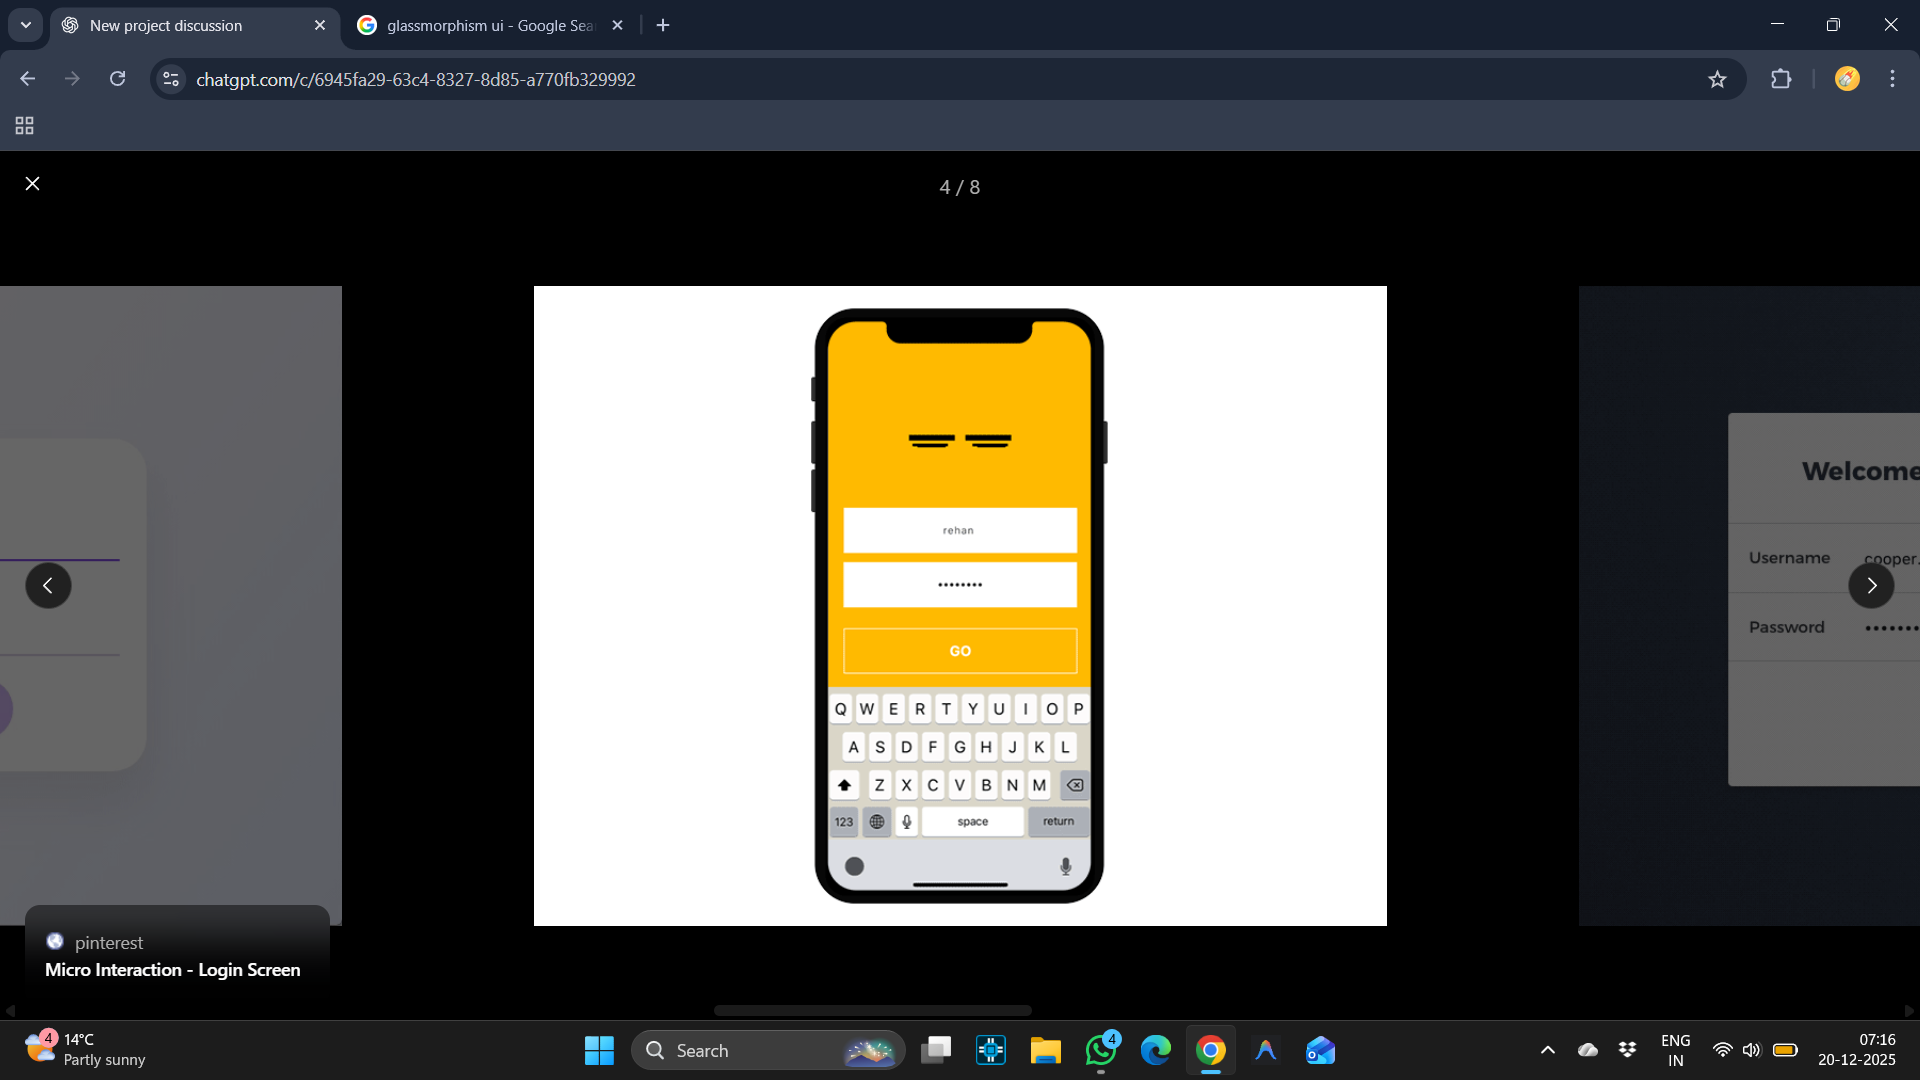
\includegraphics[width=0.7\textwidth]{images/ch_img_fc8c8209.png}
\caption{bhjn}
\end{figure}


\section{Work Process and Methodology}


\section{Key Project and Case Study}

One major project involved developing a full stack web application:


Project Background: The goal was to create a system that handles user interaction and backend processing efficiently.


Implementation: • Designed frontend UI • Developed backend APIs • Integrated frontend and backend • Handled data flow and validation • Tested performance and stability


Outcome: The application worked successfully with proper data handling and user interaction.


The project provided valuable insights into the complete software development lifecycle, from requirements gathering and design to implementation, testing, and deployment. It demonstrated the importance of proper architecture planning, code organization, and testing strategies in building maintainable and scalable applications. The experience gained from this project has been instrumental in developing a comprehensive understanding of professional software development practices.




\section{Challenges Faced}


\section{Solutions Implemented}


% ==========================================================================
% CHAPTER 4: RESULTS AND DISCUSSION
% ==========================================================================
\chapter{RESULTS AND DISCUSSION}
\label{ch:results}


The work that was evaluated and examined during the internship is included in this chapter. This chapter presents a thorough analysis of the outcomes achieved, the learning acquired, and the overall effectiveness of the internship experience. It evaluates the deliverables produced, the skills developed, and provides a critical analysis of the entire internship journey, highlighting both the successes and areas for improvement.



\begin{figure}[H]
\centering
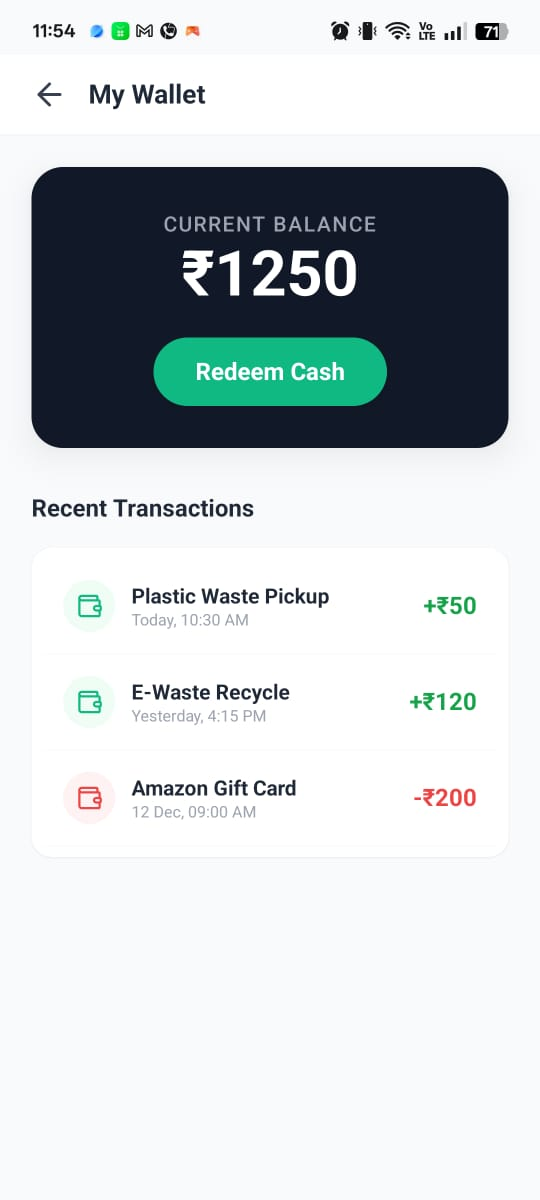
\includegraphics[width=0.7\textwidth]{images/ch_img_2ac15e60.jpg}
\caption{test}
\end{figure}


\section{Outcomes of the Work}

Key outcomes:


• Developed industrial UI dashboards • Learned embedded platforms • Worked with ROS middleware • Built full stack applications • Performed debugging using Qualcomm tools • Improved system performance • Enhanced documentation skills


These outcomes demonstrate the practical value of the internship in building real-world engineering competencies. The deliverables produced during the internship met professional quality standards and contributed meaningfully to the organization's objectives. The experience has established a strong foundation for future professional endeavors in the field.


\section{Learning Outcomes}

Learning outcomes:


• Full stack development • API integration • Embedded systems knowledge • ROS communication • Debugging and log analysis • Problem solving • System design • Technical documentation


Beyond technical competencies, the internship fostered important professional skills such as effective communication, teamwork, time management, and adaptability. These soft skills are equally valuable in a professional engineering career and complement the technical knowledge gained during the internship period.


\section{Analysis}




% ==========================================================================
% CHAPTER 5: CONCLUSION
% ==========================================================================
\chapter{CONCLUSION}
\label{ch:conclusion}


This chapter presents a comprehensive summary of the internship, the skills developed, and the path forward in the chosen domain.




\section{Summary}

Overall, my internship at Supram Technologies provided valuable exposure to multiple domains including UI design, embedded systems, and full stack development. I gained practical experience and improved my technical skills significantly.


The internship experience at Supram Technologies has been a transformative journey that has significantly enhanced both technical capabilities and professional outlook. The exposure to real-world engineering practices, combined with mentorship from experienced professionals, has provided a solid foundation for a career in technology and engineering.


\section{Personal Growth}

This internship improved my confidence, technical knowledge, and problem-solving ability. I developed a better understanding of system-level design.


The internship has instilled a growth mindset and a commitment to continuous learning. The experience of working in a professional environment has improved my ability to collaborate effectively, communicate technical concepts clearly, and approach complex problems with a structured methodology. These personal and professional developments will serve as valuable assets throughout my career.


\section{Future Scope}

This internship opens opportunities in embedded systems, full stack development, and system engineering. It provides a strong foundation for my future career.


The field continues to evolve rapidly, with emerging technologies creating new opportunities for innovation and specialization. The skills and knowledge gained during this internship provide a strong foundation for pursuing advanced studies, industry certifications, or specialized roles in technology companies. The internship has opened up multiple career pathways and has reinforced the commitment to lifelong learning in this dynamic field.


\end{document}
